\newpage


\chapter{ Guía de Usuario}
\label{chap:manual-usuario}

La aplicación RobotUI ha sido creada por Manuel López Urbina para el proyecto fin de carrera de la titulación de Ingeniería Informática de la Universidad de Cádiz.\\

Resulta de vital importancia consultar esta guía antes y/o durante la utilización de los diferentes elementos tanto hardware, robot de pruebas desarrollado, como software del presente proyecto ya 
que le proporcionará una guía paso a paso en el manejo correcto de la aplicación.\\

La resolución recomendada para la aplicación debe ser superior o igual a 1024x768 (Estándar XGA), aunque es adaptable a cualquier resolución debido a su diseño web responsive.\\

RobotUI ha sido elaborado con un claro propósito; el de  proporcionar a los usuarios un medio donde compartir sus dispositivos robóticos con el resto de usuarios. Esto es posible gracias a una serie de
herramientas desarrolladas para que, sin necesidad de tener grandes conocimientos en programación, puedan configurar un entorno para el manejo de sus proyectos robóticos y tener 
posibilidad de compartir sus dispositivos y experiencias con el resto de usuarios.\\

La particularidad de RobotUI es que el usuario propietario del robot tiene la posibilidad de permitir el manejo de sus dispositivos robóticos al resto de usuarios que él mismo considere de una 
manera controlada o, por otra parte, permitir que otros usuarios visualicen, como si de espectadores se tratase, el control que un determinado usuario realiza de un determinado robot.
Todo ello en tiempo real.\\

Por tanto, tras esta breve introducción en el ámbito de la aplicación, en este manual se describen los diferentes pasos a realizar para configurar sus dispositivos correctamente en el sistema
y abrirlo a toda una comunidad de usuarios. Además de tener abierto el acceso a otros muchos dispositivos de otras personas.\\

\subsection{Objetivo de esta guía}

Esta guía tiene como objetivo proporcionar al usuario un soporte de ayuda e iniciación a la utilización de RobotUI.\\

Esta sección comprende:\\

\begin{itemize}
 \item Introducción.
 \item Guía de acceso al código fuente de la aplicación.
 \item Guía de uso de la aplicación.
 \item Guía para la puesta en marcha y programación de un robot.
\end{itemize}

\subsection{Dirigido a}

Esta guía esta dirigida al usuario final del proyecto RobotUI. Tiene la finalidad de proporcionar una guía descriptiva de los procedimientos de creación, configuración y utilización de los diferentes dispositivos 
robóticos en sus dos modalidades disponibles, la de control y la de visualización.

\subsection{Obtener RobotUI}

El código fuente junto con la presente memoria se encuentra disponible en el repositorio GitHub en el enlace \url{https://github.com/lopi87/SAILS-RobotUI} o usando la herramienta
Git, escribiendo en la consola el siguiente comando:\\

\begin{lstlisting}[language=bash]
 git clone git@github.com:lopi87/SAILS-RobotUI.git 
\end{lstlisting}


\section{ Uso de RobotUI }
\label{sec:uso-robotui}


\subsection{ Acceso a la aplicación }
\label{sec:acceso-aplicacion}

Para acceder a la aplicación, el usuario deberá accedes al siguiente enlace: \url{www.robotui.com}. \\

Al acceder podrá ver el portal de entrada a la aplicación. En él puede acceder al resto de funcionalidades identificándose con sus credenciales y acceder a los formularios de registro
de usuario.\\

\begin{figure}[H]
  \begin{center}
    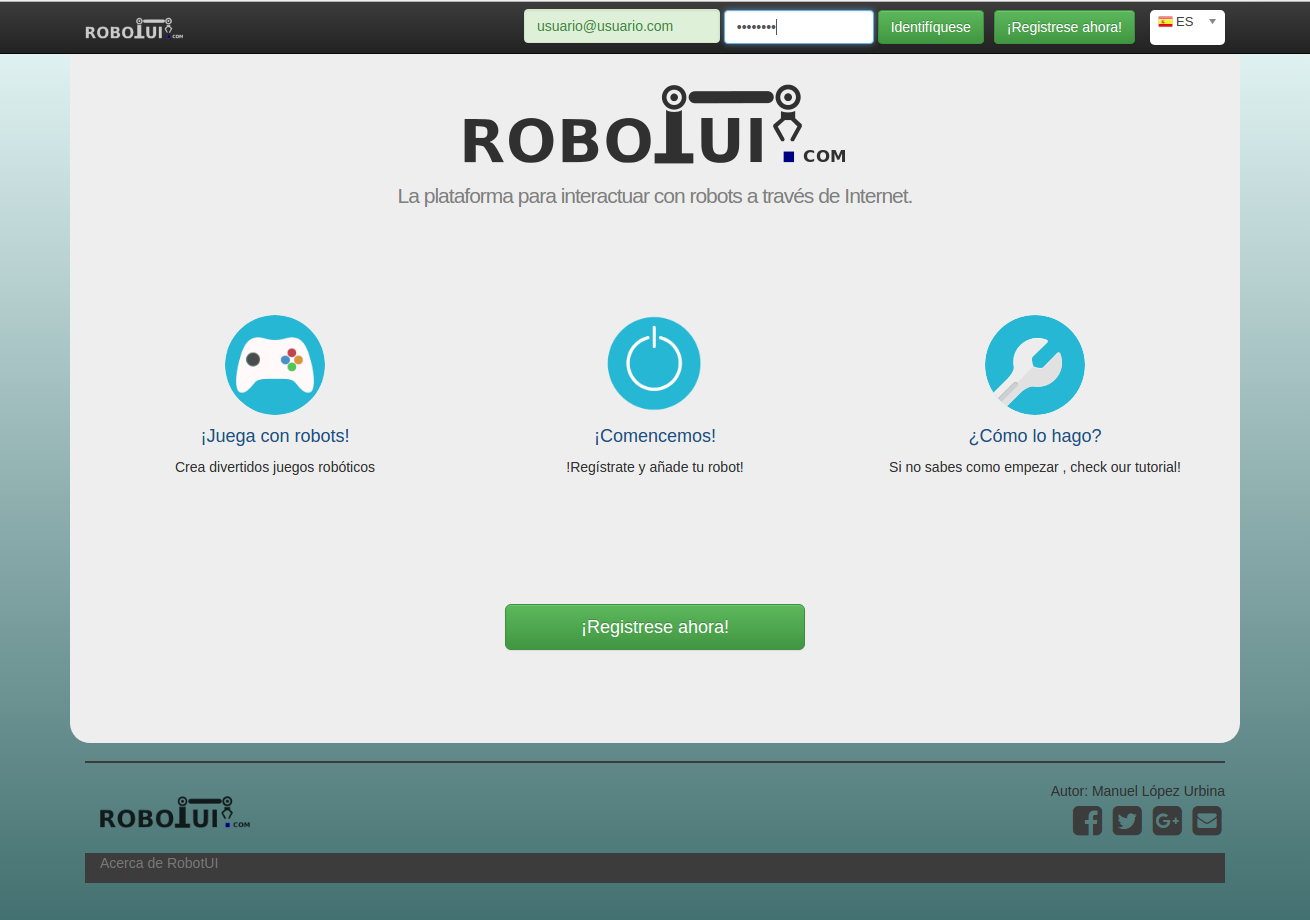
\includegraphics[scale=0.3]{imagenes/manual-usuario/pagina-principal.png}
  \end{center}
  \caption{Página principal RobotUI.}
  \label{website:pagina-principal}
\end{figure}

\subsection{ Registo de usuario }
\label{sec:creacion-usuario}

Una vez en la página principal, figura \ref{website:pagina-principal}, podemos observar la barra superior, la cual posee dos estados, la de usuario sin identificar y la de usuario identificado.

\begin{figure}[H]
  \begin{center}
    
\includegraphics[scale=0.5]{imagenes/manual-usuario/barra-menu1.png}
  \end{center}
  \caption{Vista de la barra superior en modalidad usuario no identificado en el sistema.}
  \label{website:barra-inicial}
\end{figure}

\begin{figure}[H]
  \begin{center}
    
\includegraphics[scale=0.5]{imagenes/manual-usuario/barra-menu2.png}
  \end{center}
  \caption{Vista de la barra superior en modalidad usuario identificado en el sistema.}
  \label{website:barra-usuario}
\end{figure}


Para iniciar el proceso de registro de usuario hacemos clic sobre el botón de la barra superior \icontext{.2}{.35}{imagenes/manual-usuario/btn-registro.png} mediante el cual accedemos al formulario \ref{website:formulario-registro}.

\begin{figure}[H]
  \begin{center}
    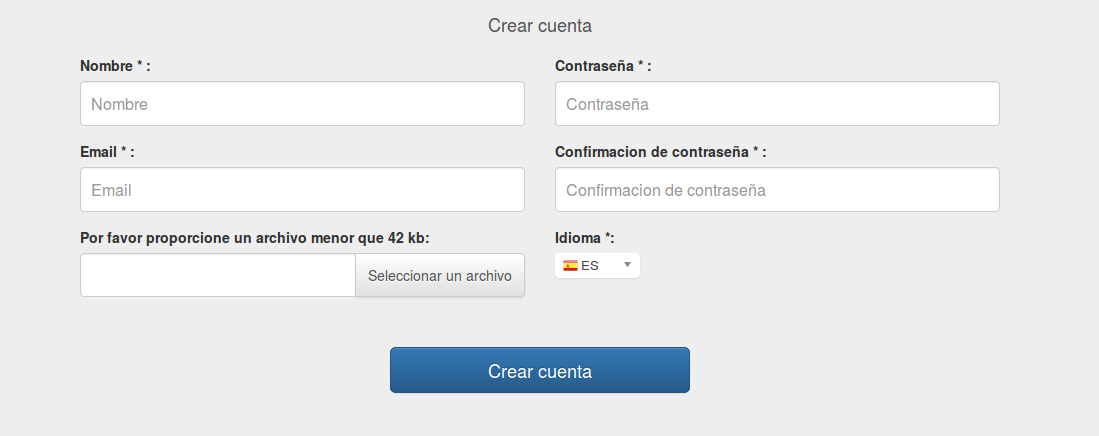
\includegraphics[scale=0.4]{imagenes/manual-usuario/pagina-registro.png}
  \end{center}
  \caption{Formulario de registro de usuario.}
  \label{website:formulario-registro}
\end{figure}

Para proceder con el registro necesitaremos los siguientes datos:

\begin{enumerate}
 \item Nombre: nombre de usuario.
 \item Email: dirección de correo electrónico utilizada para acceder al sistema.
 \item Contraseña: deberá proporcionar una contraseña para poder acceder al sistema.
 \item Confirmación de contraseña: campo para comprobar que la contraseña es la deseada por el usuario.
 \item Imagen: imagen avatar del usuario.
 \item Idioma: selección del idioma por defecto del usuario.
\end{enumerate}

Una vez introducidos los datos correctamente podremos hacer clic en \emph{crear cuenta}. Si los datos introducidos son correctos dispondremos de un nuevo usuario en la aplicación redirigiéndonos
a la página de información del nuevo usuario
\ref{website:informacion-usuario}.

\begin{figure}[H]
  \begin{center}
    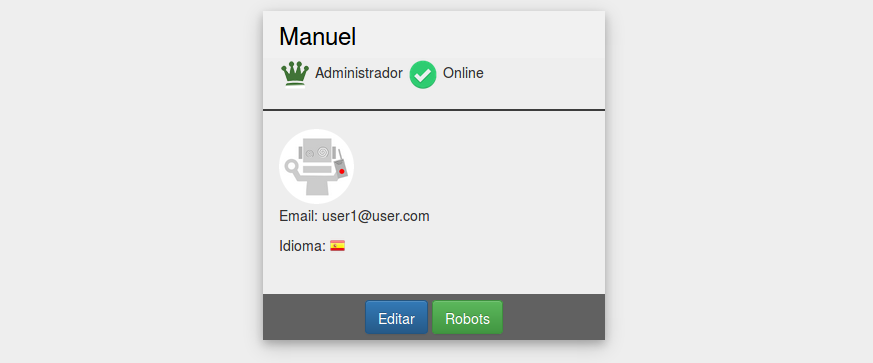
\includegraphics[scale=0.4]{imagenes/manual-usuario/informacion-usuario.png}
  \end{center}
  \caption{Información de un usuario.}
  \label{website:informacion-usuario}
\end{figure}



\subsection{ Ingreso al sistema }
\label{sec:ingreso-sisetma}

Una vez registrados, procedimiento descrito en \ref{sec:creacion-usuario}, podremos acceder al sistema mediante la introducción de nuestro usuario y contraseña en los campos disponibles en la barra
superior localizado en la aplicación y haciendo clic en \icontext{.2}{.45}{imagenes/manual-usuario/btn-identifiquese.png} localizados en la barra superior.\\

\subsection{Registro de un Robot}
\label{sec:creacion-robot}

Para el iniciar el proceso de creación de un robot haremos clic en \emph{Robots} \textrightarrow \enspace \emph{Mis robots} del menú superior accediendo al formulario de creación, figura
\ref{website:creacion-robot}.\\

En este caso registraremos nuestro robot de pruebas descrito en el capítulo \ref{chap:robot}. Para ello introducimos los siguientes datos:\\

\begin{enumerate}
 \item \textbf{Nombre:} nombre de nuestro robot.
 \item \textbf{Dirección IP:} dirección donde se encontrará accesible nuestro robot.
 \item \textbf{Puerto:} puerto donde se encontrará nuestro robot a la escucha de conexiones.
 \item \textbf{Descripción:} campo opcional en el que podemos añadir una descripción de nuestro robot y que será visible al resto de usuarios.
 \item \textbf{Imagen:} campo opcional en el que podremos subir una imagen de nuestro robot.
 \item \textbf{Usuarios espectadores:} selector en el que podemos especificar qué usuarios del sistema tendrán permisos para visualizar el funcionamiento de nuestro robot.
 \item \textbf{Usuarios controladores:} selector para especificar qué usuarios podrán tomar control de nuestro robot.
 \item \textbf{Público:} checkboxes para indicar si por el contrario, el robot que abierto a todos los usuarios para su control o abierto para su visualización si marcamos el primero o el segundo checkbox respectivamente
 y haciendo por tanto inválidos los parámetros de los selectores anteriores.
\end{enumerate}

Una vez introducidos los datos para el nuevo usuario pulsamos en \icontext{.2}{.35}{imagenes/manual-usuario/btn-crear.png}.\\

\begin{figure}[H]
  \begin{center}
    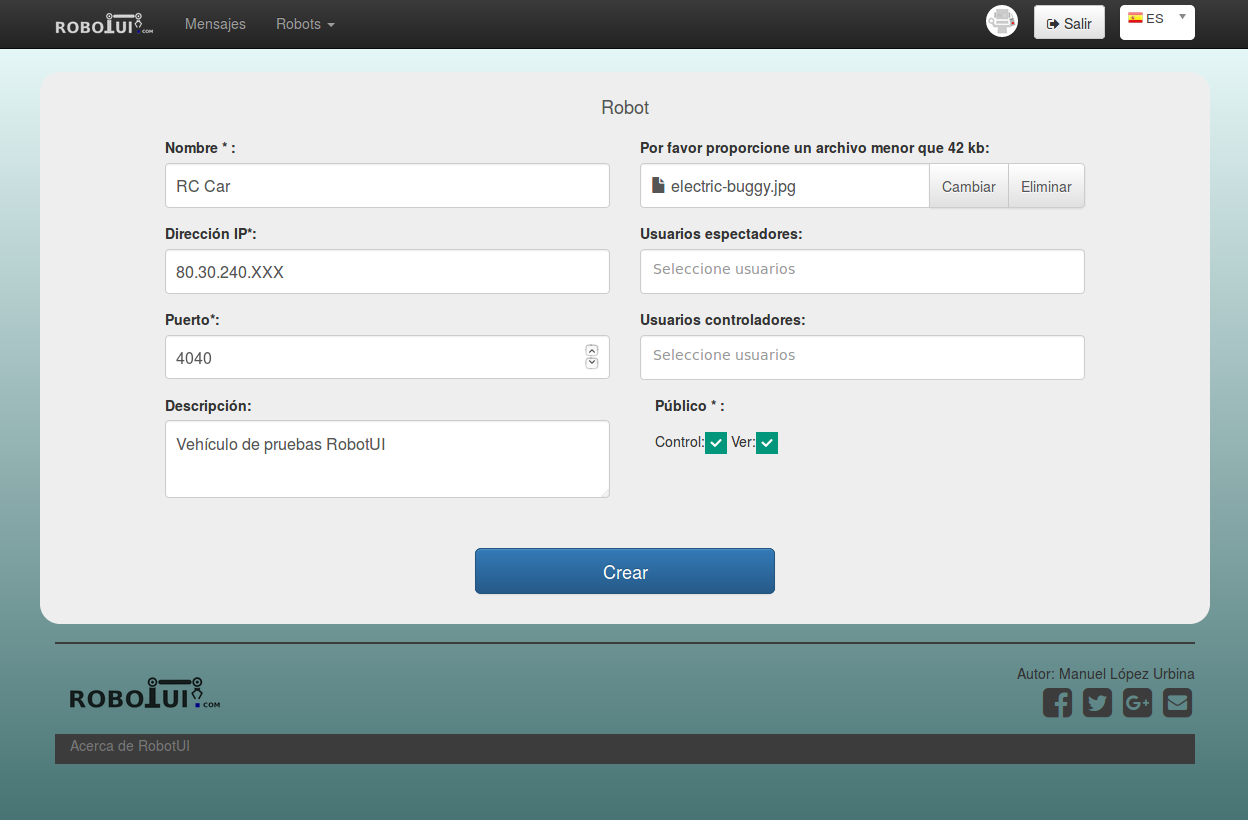
\includegraphics[scale=0.3]{imagenes/manual-usuario/pagina-crear-robot.png}
  \end{center}
  \caption{Formulario de creación de un robot.}
  \label{website:creacion-robot}
\end{figure}


Si los campos introducidos son correctos la aplicación nos redireccionará a la página informativa de nuestro nuevo robot:\\

\begin{figure}[H]
  \begin{center}
    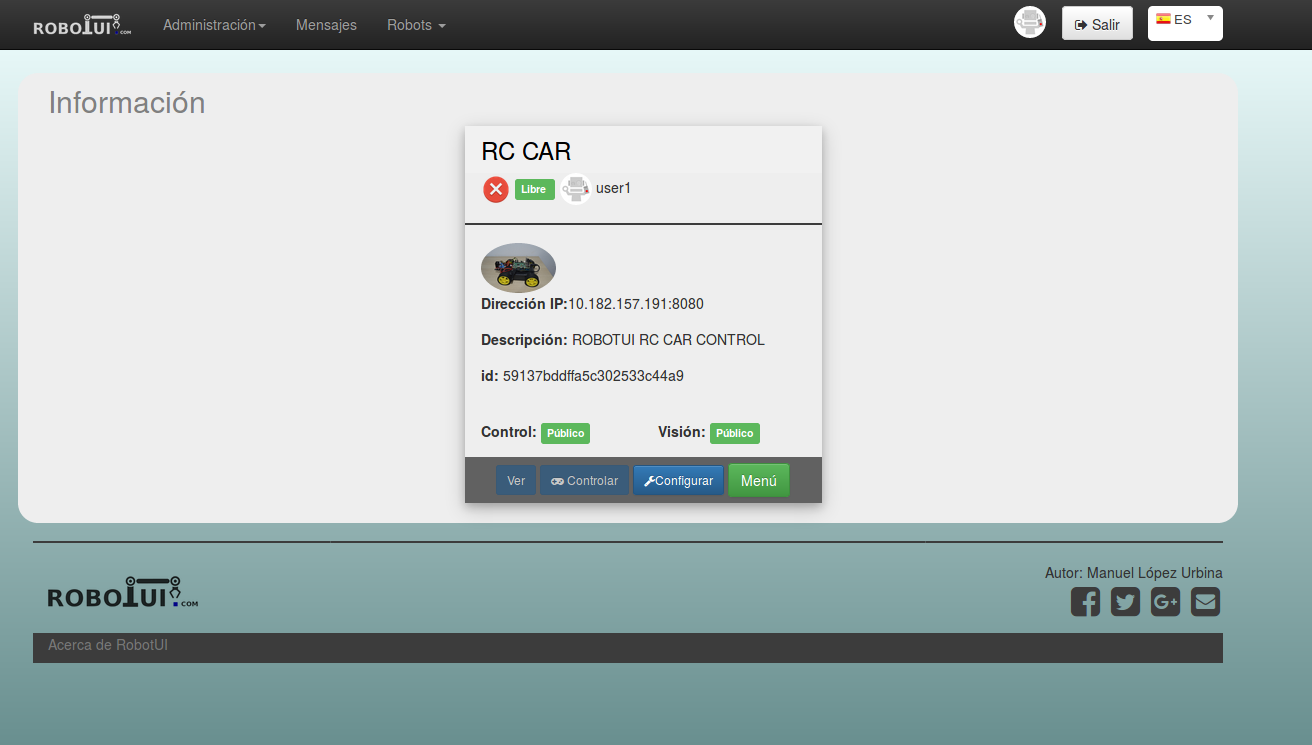
\includegraphics[scale=0.3]{imagenes/manual-usuario/show-robot.png}
  \end{center}
  \caption{Vista informativa de un robot.}
  \label{website:show-robot}
\end{figure}

En la ventana informativa de un robot, figura \ref{website:show-robot}, podemos apreciar una serie de elementos representativos de los diferentes estados en los que se puede encontrar el dispositivo. La 
tabla \ref{table:robot-estados} describe cada uno de los elementos:\\

\begin{table}[H]
  \begin{center}
    \begin{tabular}{|p{2cm}|p{10cm}|}
      \hline
      \centering{Elemento} & \qquad \quad Significado \\
      \hline
      
\includegraphics[width=1cm]{imagenes/manual-usuario/offline.png} & Imagen indicativa de estado \emph{offline}. El robot se encuentra sin conexión. \\
      \hline
      
\includegraphics[width=1cm]{imagenes/manual-usuario/online.png} & Imagen indicativa de estado \emph{online}. El robot se encuentra conectado, reemplazará a la imagen de estado \emph{offline}. \\
      \hline
      
\includegraphics[width=2cm]{imagenes/manual-usuario/control-publico.png} & Imagen representativa de robot de control público. \\
      \hline
      
\includegraphics[width=2cm]{imagenes/manual-usuario/control-privado.png} & Imagen representativa de robot de control privado. \\
      \hline
      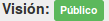
\includegraphics[width=2cm]{imagenes/manual-usuario/vision-publico.png} & Imagen representativa de robot de seguimiento pública. \\
      \hline
      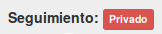
\includegraphics[width=2.2cm]{imagenes/manual-usuario/seguimiento-privado.png} & Imagen representativa de robot de seguimiento privado. \\
      \hline
      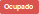
\includegraphics[width=2.2cm]{imagenes/manual-usuario/ocupado.png} & Imagen representativa de robot en uso. \\
      \hline
    \end{tabular}
  \end{center}
\caption{Elementos representativos de los estados de un robot junto con su descripción.}
\label{table:robot-estados}
\end{table}


\subsection{Gestión de permisos}

Como hemos mencionado en el procedimiento de registro de un robot, éste se puede crear con una serie de permisos. Existen dos modalidades en RobotUI, como sabemos, la de visualización o seguimiento
y la de control. Funcionalidades que podemos hacer públicas o privadas, y, en el caso de que optemos por alguna modalidad privada, definir para qué usuarios estará disponible.\\

La gestión y visualización de los permisos configurados estarán disponibles en todo momento en la ventana de edición de un robot. En ella podremos visualizar los diferentes usuarios añadidos con
los permisos de cada uno de ellos. Podremos eliminar usuarios o añadir otros nuevos estableciendo el acceso a alguna de las modalidades existentes como pública o privada.\\

Si el robot es establecido como público en alguna de sus dos modalidades (control o seguimiento) entonces se ignorará toda la configuración de usuarios establecida para esa modalidad aunque
permanecerán registradas en el sistema por si se desea volver al modo privado tan solo haciendo clic en el checkbox correspondiente.\\

\begin{figure}[H]
  \begin{center}
    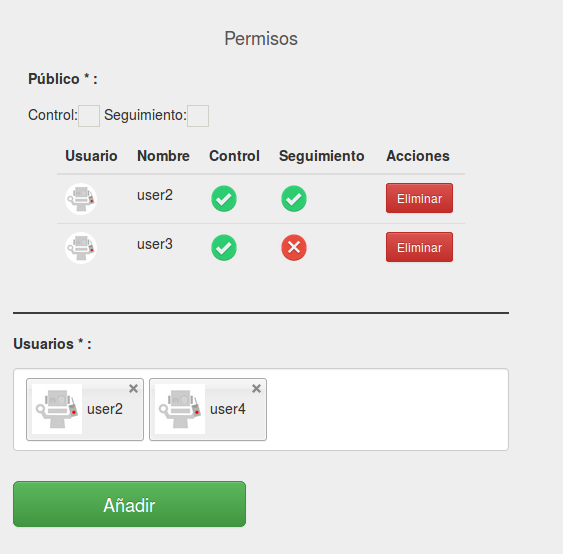
\includegraphics[scale=0.5]{imagenes/manual-usuario/panel-permisos.png}
  \end{center}
  \caption{Panel de configuración de los permisos de un robot.}
  \label{website:creacion-robot}
\end{figure}


\begin{figure}[H]
    \centering
    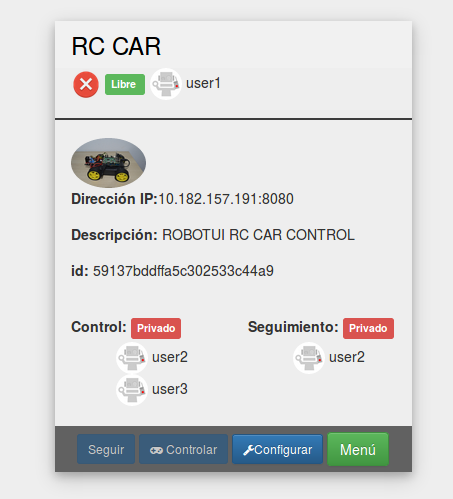
\includegraphics[width=6cm]{imagenes/manual-usuario/robot-privado.png}
    \qquad
    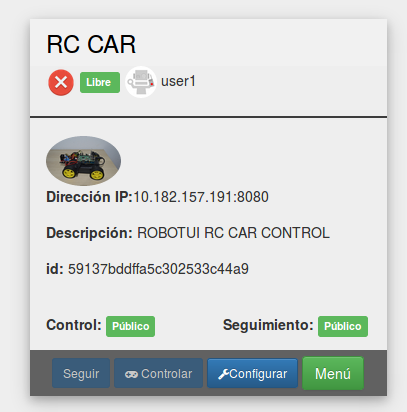
\includegraphics[width=6.5cm]{imagenes/manual-usuario/robot-publico.png}
    \caption{Panel informativo de un robot privado frente a uno público.}%
    \label{fig:http-request}%
\end{figure}


\subsection{Configuración de la interfaz}
\label{subsec:configuracion-interfaz}

Una vez creado nuestro robot en el sistema ya podremos configurar su interfaz. En la figura \ref{website:configuracion-interfaz} podemos ver el canvas sobre el que iremos añadiendo los diferentes elementos que 
conformarán nuestro panel de control. \\

El diseño resultante de esta ventana servirá tanto para panel de control del robot como ventana de seguimiento a los usuarios que sigan el funcionamiento del
dispositivo.\\

\begin{figure}[H]
  \begin{center}
    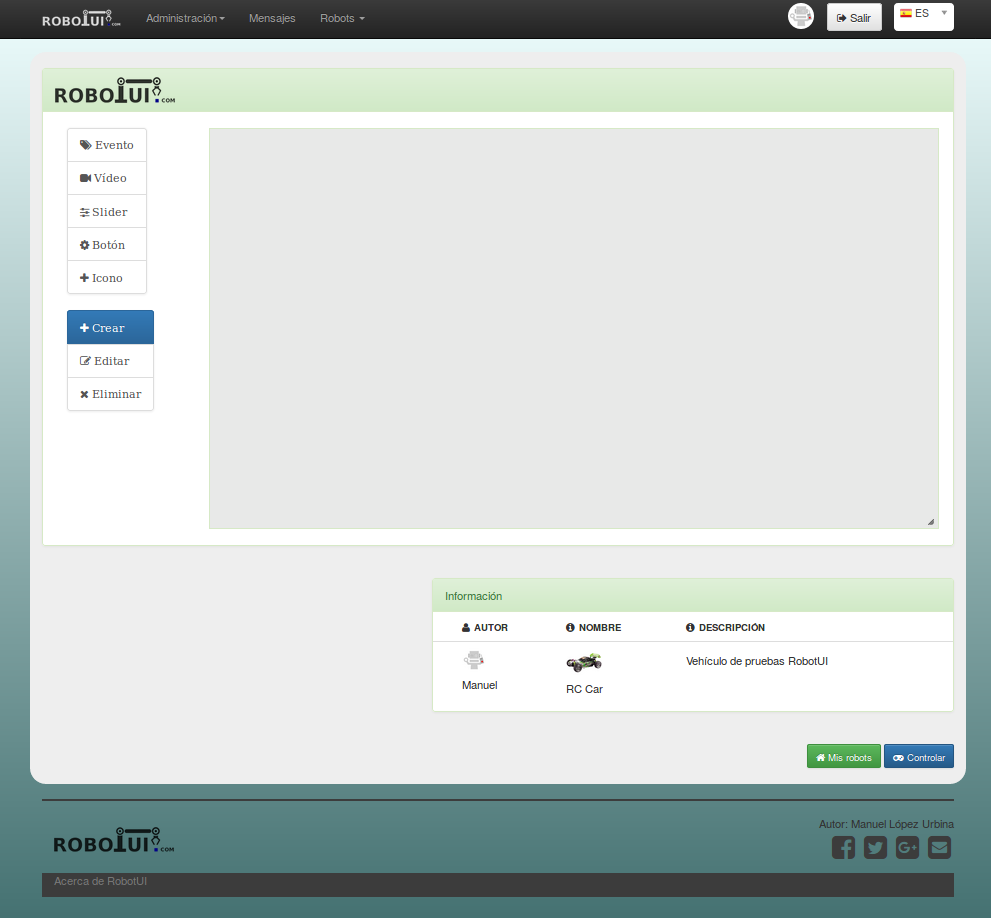
\includegraphics[scale=0.4]{imagenes/manual-usuario/pagina-configurar-interfaz.png}
  \end{center}
  \caption{Panel de configuración de la interfaz sin elementos añadidos.}
  \label{website:configuracion-interfaz}
\end{figure}

La figura \ref{website:configuracion-interfaz} correspondiente al panel de configuración de una interfaz queda dividida en los siguientes elementos:

\begin{enumerate}
  \item Panel de elementos disponibles (Evento, Vídeo, Slider, Botón e Icono).
 \item Panel de acciones sobre elementos (Crear, editar y eliminar).
 \item Panel canvas sobre el que posicionar los elementos.
 \item Panel informativo de las características del robot.
\end{enumerate}


\begin{figure}[H]
  \begin{center}
    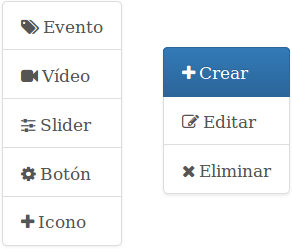
\includegraphics[scale=.6]{imagenes/manual-usuario/barra-herramientas-interfaz.png}
  \end{center}
  \caption{Panel de elemento (izquierda) y panel de acciones (derecha) para la configuración de la interfaz.}
  \label{website:pagina-principal}
\end{figure}


En los siguientes subapartados se describen los procedimientos para la creación, edición y borrados de elementos:\\


\subsubsection{Nuevo elemento}

 Para la creación de elementos debemos tener seleccionado el modo creación en el panel de acciones y pulsar sobre el tipo de nuevo elemento deseado. La siguiente tabla muestra las diferentes combinaciones:
  
\begin{table}[H]
  \begin{center}
    \begin{tabular}{|p{2cm}|p{2cm}|p{10cm}|}
      \hline
      \centering{\textbf{Botón}} & \centering{\textbf{Modo}} & \qquad \quad \textbf{Acción} \\
      \hline
      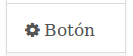
\includegraphics[width=2cm]{imagenes/manual-usuario/nuevo-boton.png} & 
\includegraphics[width=2cm]{imagenes/manual-usuario/btn-new.png} & Apertura del formulario para la creación de un botón. \\
      \hline
      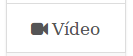
\includegraphics[width=2cm]{imagenes/manual-usuario/nuevo-video.png} & 
\includegraphics[width=2cm]{imagenes/manual-usuario/btn-new.png} & Apertura del formulario para la creación de un canvas de vídeo. \\
      \hline
      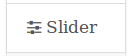
\includegraphics[width=2cm]{imagenes/manual-usuario/nuevo-slider.png} & 
\includegraphics[width=2cm]{imagenes/manual-usuario/btn-new.png} & Apertura del formulario para la creación de un slider. \\
      \hline
      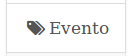
\includegraphics[width=2cm]{imagenes/manual-usuario/nuevo-evento.png} & 
\includegraphics[width=2cm]{imagenes/manual-usuario/btn-new.png} & Apertura del formulario para la creación de una etiqueta. \\
      \hline
      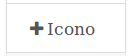
\includegraphics[width=2cm]{imagenes/manual-usuario/nuevo-icono.png} & 
\includegraphics[width=2cm]{imagenes/manual-usuario/btn-new.png} & Apertura del formulario para la subida de un icono. \\
      \hline
    \end{tabular}
  \end{center}
\caption{Elementos añadibles a una interfaz.}
\end{table}


Una vez completado el formulario y creado el nuevo elemento tan solo debemos arrastrar el nuevo elemento a la posición deseada.


\begin{figure}[H]
  \begin{center}
    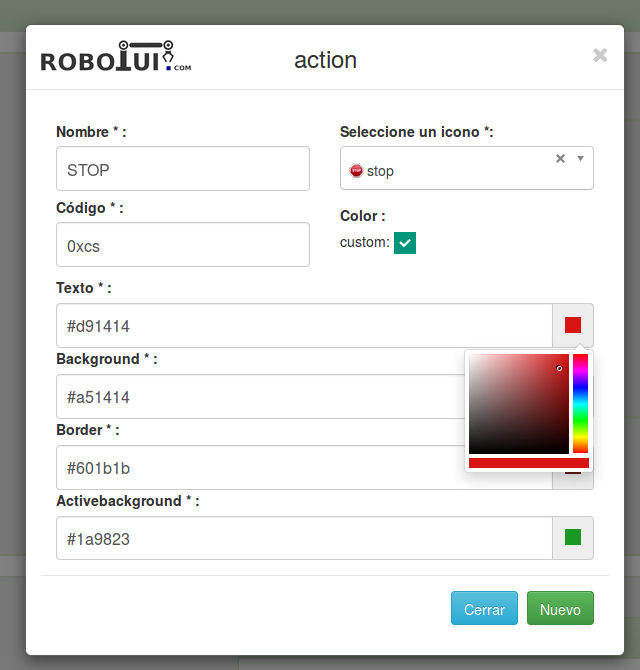
\includegraphics[scale=.4]{imagenes/manual-usuario/formulario-action.png}
  \end{center}
  \caption{Formulario para la creación de un botón.}
  \label{website:pagina-principal}
\end{figure}

Del mismo modo para la creación del resto de tipos de elementos.

\subsubsection{Editar elemento}

Para la edición de elementos pulsaremos seleccionaremos el modo edición \icontext{.2}{.35}{imagenes/manual-usuario/btn-edit.png} y posteriormente haremos clic sobre el elemento que deseemos editar.\\

Tras ello se abrirá el formulario correspondiente, modificamos los parámetros deseados y pulsamos guardar.\\

\subsubsection{Eliminar elemento}

Del mismo modo que en la edición de elementos, para borrar un elemento seleccionaremos el modo eliminar \icontext{.2}{.35}{imagenes/manual-usuario/btn-destroy.png}  del panel de acciones y posteriormente haremos clic sobre el elemento que deseemos borrar.\\


\subsection{Ejemplo}

La figura \ref{interfaz-configurada} muestra una posible interfaz de control para un dispositivo robótico.

\begin{figure}[H]
  \begin{center}
    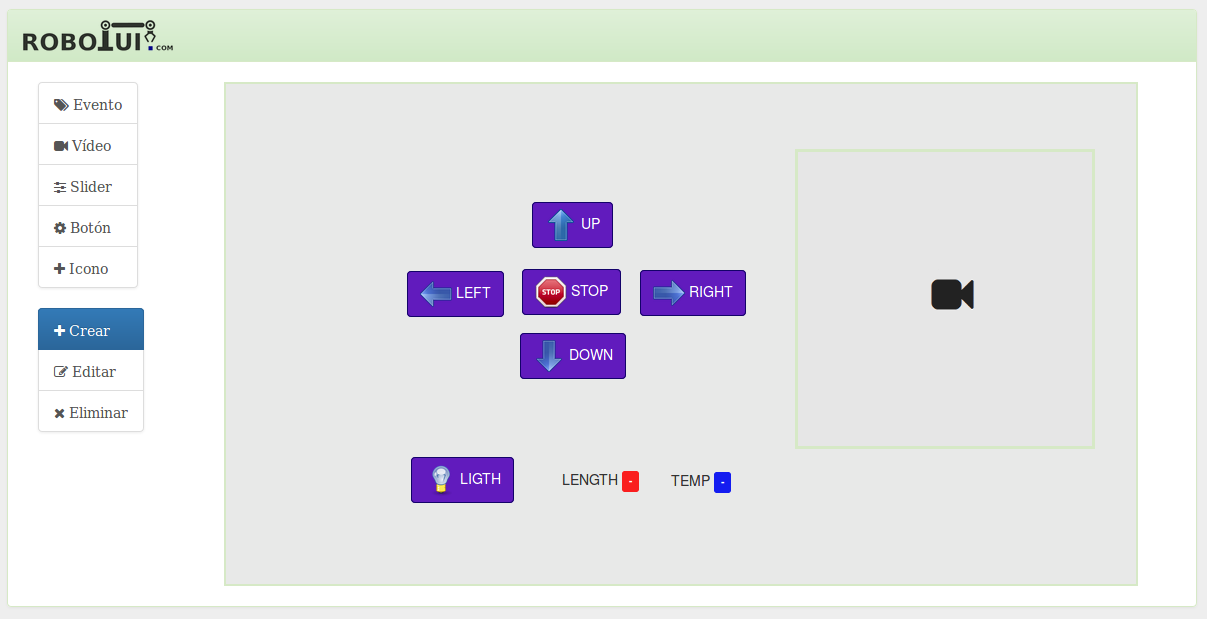
\includegraphics[scale=.4]{imagenes/manual-usuario/interfaz-creada.png}
  \end{center}
  \caption{Vista tipo de una interfaz configurada.}
  \label{website:interfaz-configurada}
\end{figure}



\section{ Programa tu robot }
\label{sec:programacion-robot}

NOTA: Esta guía comprende una serie de pasos para realizar la programación de un dispositivo robótico para la aplicación RobotUI. En este caso particular, el robot empleado posee como base una placa 
Raspberry Pi, la cual emplea para la conexión de sensores y motores haciendo uso de su sistema de Entrada/Salio Gpio.\\

El sistema es compatible con cualquier dispositivo, no solo limitado a las placas Raspberry. La única diferencia radica en que se deberán emplear a nivel de programación las bibliotecas adecuadas 
para la activación o lectura de las Entadas/Salidas correspondientes al modelo de placa utilizado.\\

Antes de proceder con la programación de nuestro robot debemos de realizar su creación en la aplicación RobotUI como queda descrito en el punto \ref{sec:creacion-robot} y 
tomar nota del identificador único que la aplicación proporciona para dicho robot y que posteriormente necesitaremos.\\	

\begin{figure}[H]
  \begin{center}
    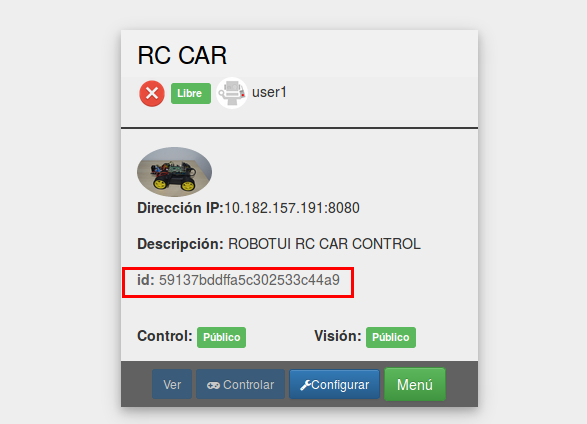
\includegraphics[scale=.6]{imagenes/manual-usuario/identificador.png}
  \end{center}
  \caption{Panel informativo de un robot donde se aprecia su identificador.}
  \label{website:pagina-principal}
\end{figure}


Una vez creado el robot y configurada su interfaz, añadiendo los diferentes elementos disponibles como acciones, vídeo, etiquetas, etcétera, recogidos en el punto \ref{subsec:configuracion-interfaz}: Configuración de la interfaz.
Podemos comenzar con la programación del robot.\\

Para ello debemos seguir una serie de pasos:\\

\begin{enumerate}
  \item Generar una archivo de extensión .js, con el código base mostrado en el punto \ref{codigo:base}.
  \item Reemplazar en el código la palabra \emph{IDENTIFICADOR} por el identificador único de nuestro robot obtenido en la vista informativa del mismo.
  Por ejemplo: 59188631c8e94ba54f7a4bdc.
  \item Indicar el puerto en el que el robot permanecerá a la escucha. Para ello debemos reemplazar palabra \emph{PUERTO} del código inferior por el puerto deseado. Por ejemplo 8085. 
  \item El siguiente paso es es determinar qué puertos GPIO necesitaremos y si van a ser utilizado en modo Entrada, Salida o Entrada/Salida dentro de la sección \emph{PINES} de la plantilla.
  En este caso se ha empleando la biblioteca \emph{pigpio} cuya documentación se encuentra disponible en el siguiente enlace: \url{https://www.npmjs.com/package/pigpio}.
  \item Definir el funcionamiento de los diferentes eventos dentro de la sección \emph{EVENTOS}.
\end{enumerate}


\subsubsection{código base}
\label{codigo:base}

\begin{lstlisting}[language=JavaScript]

var io_client = require('./node_modules/socket.io-client');
var sails_client = require('./node_modules/sails.io.js');
var io_server = sails_client(io_client);
io_server.sails.url = 'http://46.101.102.33:80';
io_server.socket.get('/robot/changetoonline/', {robot: 'IDENTIFICADOR', online: true});

// Inicia servidor socket.io en el puerto PUERTO.
var io =io_client.listen( PUERTO, { log: false });

var ffmpeg_command, running_camera = false, child_process = require('child_process');

var Gpio = require('pigpio').Gpio;


// SECCION PINES 

// EJEMPLO: 
//      var gpio2 = new Gpio(2, {mode: Gpio.OUTPUT}),
//	    gpio3 = new Gpio(3, {mode: Gpio.OUTPUT}),
//	    gpio17 = new Gpio(17, {mode: Gpio.OUTPUT}),
//	    gpio27 = new Gpio(27, {mode: Gpio.OUTPUT});


// FIN SECCION PINES


console.log('Esperando conexión...');

var sockets = {};

io.sockets.on('connection', function (socket)
{

    // SECCION EVENTOS

    // FIN SECCION EVENTOS
});

function stopStreaming(socket) {
  delete sockets[socket.id];
  // no more sockets, kill the stream
  if (Object.keys(sockets).length == 0) {
    if (ffmpeg_command){
      ffmpeg_command.kill();
      running_camera = false;
      console.log('Stop streaming');
    }
  }
}

function startStreaming(socket) {
  if (running_camera == false){
    console.log('Starting streaming....');
    var args = ["-f", "video4linux2", "-i", "/dev/video0", "-s", "300x150","-f","mjpeg", "pipe:1", "-b:v 28k", "-bufsize 28k"]
    ffmpeg_command = child_process.spawn("ffmpeg", args);
    running_camera = true
  }

  ffmpeg_command.on('error', function(err, stdout, stderr) {
    console.log("ffmpeg stdout:\n" + stdout);
    console.log("ffmpeg stderr:\n" + stderr);
    running_camera = false
  });


  ffmpeg_command.on('close', function (code) {
    console.log('ffmpeg exited' + code );
    running_camera = false
  });


  ffmpeg_command.stderr.on('data', function (data) {
    //console.log('stderr: ' + data);
  });

  ffmpeg_command.on('end', function() {
    console.log('Fin');
    running_camera = false
  });

  ffmpeg_command.stdout.on('data', function (data) {
    //console.log('stdout: ' + data);
    var frame = new Buffer(data).toString('base64');
    socket.emit('canvas',frame);
  });

}

\end{lstlisting}

A continuación mostramos dos posibles eventos para añadir al código base superior a modo orientativo:\\

El primer fragmento de cógigo se activa al recibir un evento tipo \emph{action} (evento lanzado desde la interfaz al presionar cualquier botón generado por el usuario), captura el comando recibido,
y si es igual a \emph{UP}, entonces habilita el pin gpio1 con el valor 1. Pin inicializado previamente en la sección de pines del código base.\\

\begin{lstlisting}[language=JavaScript]

socket.on('action', function (data){
    if (data == 'UP') {
        gpio1.digitalWrite(1);
    }
});

\end{lstlisting}

El segundo fragmento de código devuelve la lectura del pin \emph{gpio2} cada vez que recibe el comando \emph{READ} y mandando al cliente el valor de lectura obtenido:\\

\begin{lstlisting}[language=JavaScript]

  socket.on('action', function (data){
      if (data == 'READ') {
	var temp =  gpio2.digitalRead(1);
	socket.emit('robot_temp', {msg: temp});
    }
  });
\end{lstlisting}
 

En la parte referente a la interfaz de control de la aplicacion RobotUI, para lanzar o capturar los comandos correspondientes a los ejemplos superiores, en el primer caso, debemos crear un botón 
cuyo código a emitir sea \emph{UP} y para el segundo, debemos añadir un botón cuyo código de emisión sea \emph{READ} y una etiqueta cuyo nombre de evento se cprresponda con \emph{robot\_temp}.\\

Una vez generado el código para nuestro robot debemos copiarlo a la placa Raspberry Pi o computador que actuará como Robot para nuestra aplicación y ejecutarlo. Para la ejecución del código
introducimos el siguiente comando:\\

\begin{lstlisting}[language=bash]
  sudo node raspberry.js
\end{lstlisting}

Siendo \emph{raspberry.js} el nombre del archivo que contiene nuestro código.


Obteniendo el siguiente resultado:


\begin{figure}[H]
  \begin{center}
    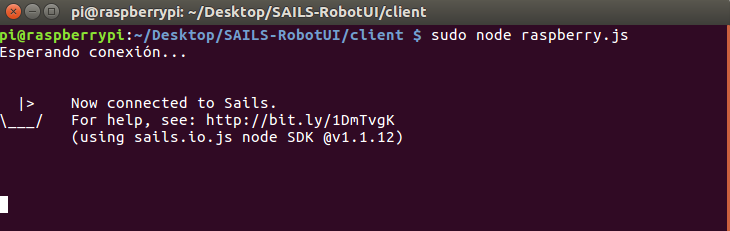
\includegraphics[scale=.6]{imagenes/manual-usuario/espera-conexion.png}
  \end{center}
  \caption{ Robot a la espera de conexión entrante.}
  \label{website:pagina-principal}
\end{figure}



\section{ Controla tu robot }
\label{sec:control-robot}

El panel de control de la interfaz podemos identificar los siguientes elementos:

\begin{figure}[H]
  \begin{center}
    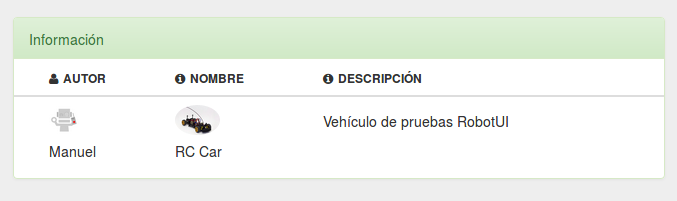
\includegraphics[scale=.6]{imagenes/manual-usuario/panel-robot-info.png}
  \end{center}
  \caption{ Panel informativo de las características del robot de la interfaz.}
  \label{website:pagina-principal}
\end{figure}


\begin{figure}[H]
  \begin{center}
    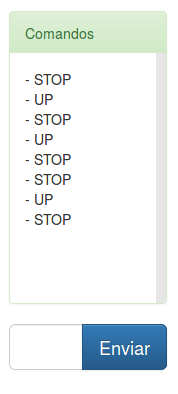
\includegraphics[scale=.6]{imagenes/manual-usuario/panel-comandos.png}
  \end{center}
  \caption{ Panel informativo de las órdenes enviadas al robot junto con una entrada de comandos para enviar nuevas órdenes directamente.}
  \label{website:pagina-principal}
\end{figure}


\section{ Visita otros robots }
\label{sec:visita-robot}


En la aplicación accediendo desde el menú superior en el desplegable robots -> públicos podemos acceder en todo momento a los robots que tenemos accesibles.

\begin{figure}[H]
  \begin{center}
    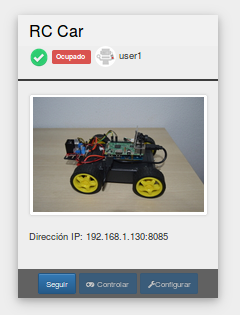
\includegraphics[scale=.6]{imagenes/manual-usuario/tarjeta_ocupado.png}
  \end{center}
  \caption{ Panel informativo de un robot en su modalidad \emh{ocupado}.}
  \label{website:robot-ocupado}
\end{figure}

Para pulsamos sobre el botón seguir accediendo a su interfaz en modo espectador mostrando una vista similar a la de la figura \ref{website:ventana-seguimiento}:\\

\begin{figure}[H]
  \begin{center}
    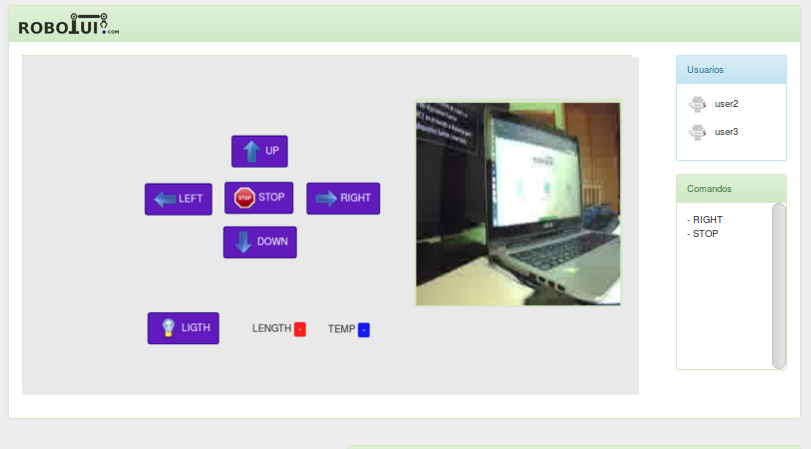
\includegraphics[scale=.6]{imagenes/manual-usuario/vista_seguimiento.png}
  \end{center}
  \caption{ Vista del panel de seguimiento de un robot en tiempo real.}
  \label{website:ventana-seguimiento}
\end{figure}


El usuario que dispone del control del robot verá lo siguiente:


\begin{figure}[H]
  \begin{center}
    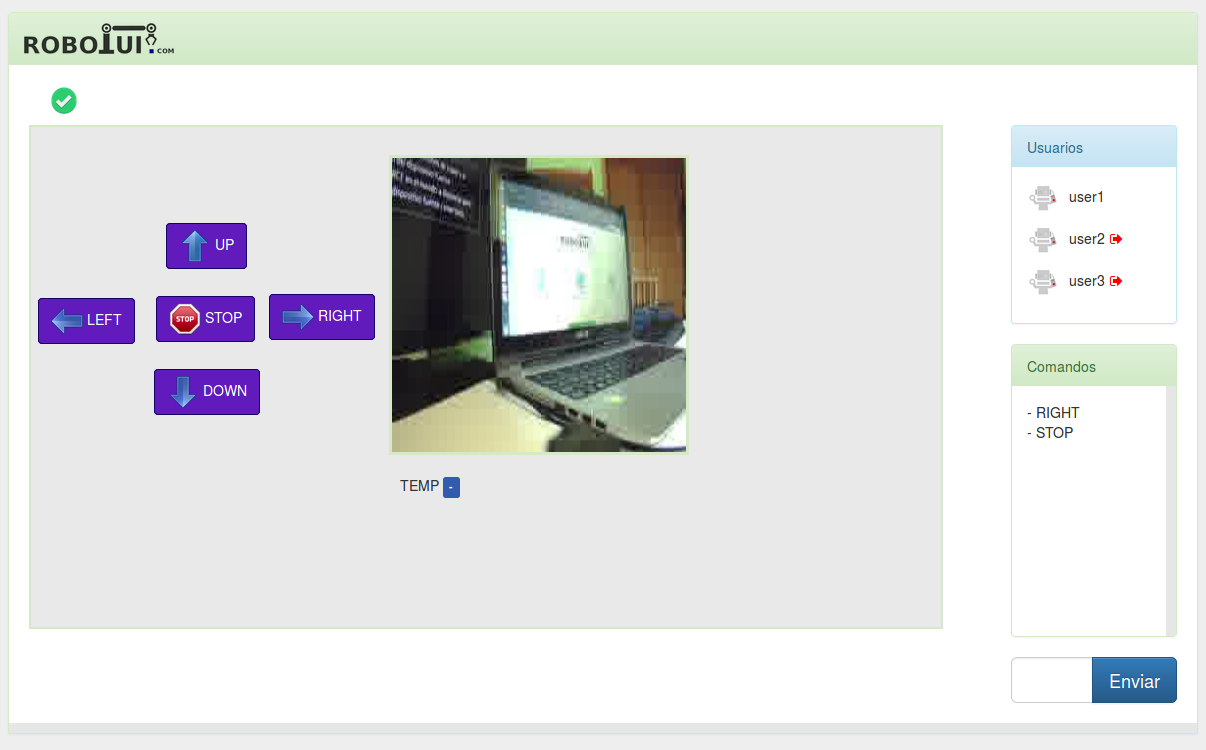
\includegraphics[scale=.4]{imagenes/manual-usuario/vista_control.png}
  \end{center}
  \caption{ Vista del panel de control de un robot junto con el listado de usuarios realizando el seguimiento.}
  \label{website:ventana-seguimiento}
\end{figure}



\begin{figure}[H]
  \begin{center}
    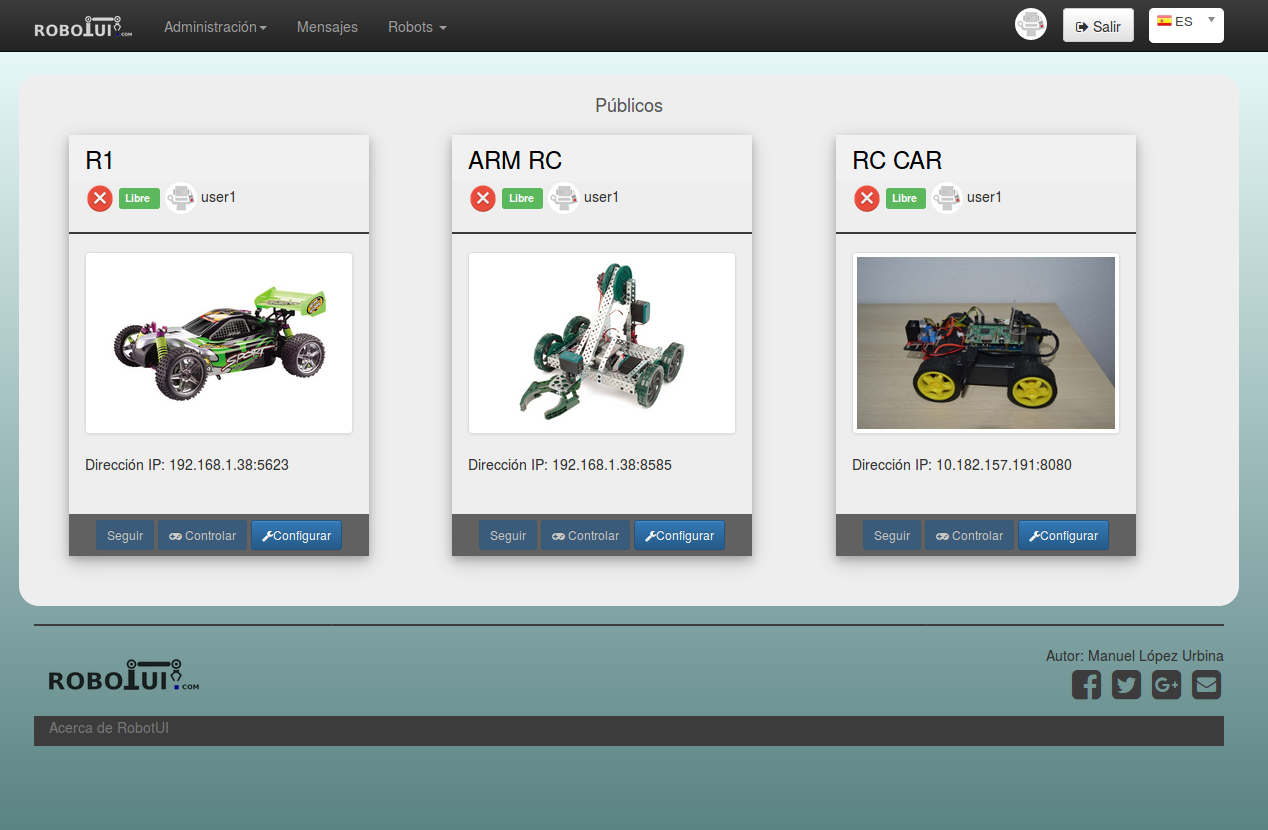
\includegraphics[scale=.35]{imagenes/manual-usuario/robots-publicos.png}
  \end{center}
  \caption{ Vista de acceso a los robots públicos.}
  \label{website:pagina-principal}
\end{figure}




\subsection{Panel de administración}


Menú accesible solo para usuarios administradores. Accesible desde la barra superior disponiendo de la entrada \emph{Usuarios} y \emph{Robots}.

